%%%%%%%%%%%%%%%%%%don't forget if needed %%%%%%%%%%%%%%%%%%%%%
%\section[toc version]{title version%
%              \sectionmark{head version}}
%\sectionmark{head version}
%%%%%%%%%%%%%%%%%%%%%%%%%%%%%%%%%%%%%%%%%%%%%%%%%%%%%%%%%%%%%%
\def\titcourt{Introduction}
\def\titlong{Introduction}
%%%%%%%%%%%%%%%%%%%%%%%%%%%%%%%%%%%%%%%%%%%%%%%%%%%%%%%%%%%%%%%%
\chapter[\titlong]{\titlong%
              \chaptermark{\titcourt}}
\chaptermark{\titcourt}
%%%%%%%%%%%%%%%%%%%%%%%%%%%%%%%%%%%%%%%%%%%%%%%%%%%%%%%%%%%%%%%%
%%%%%%%%%%%%%%%%%%%%%%%%%%%%%%%%%%%%%%%%%%%%%%%%%%%%%%%%%%%%%%%%

\section{Phase change materials}

Interest in renewable and sustainable energy sources is increasing nowadays. 
In the past decades, the world's energy consumption was fully dominated by fossil fuels such as coal, natural gas or raw oil.
Fig. \ref{fig-Energ-cons}a illustrate the energy sources for electricity generation by seven region in the world in 2017.
It is clearly shown that coal and natural gas are the main energy used. 
Today, we must face to the fact that these fossil fuels are going to an end.
Moreover, their large utilization has induced considerable impacts on our environment.
Notwithstanding until today, our dependency on those energy sources is still causing severer environmental issues.
Climate changing, mostly due to the huge CO2 and other green house gases released into the atmosphere, is more than ever experienced in our daily life:
unnatural heat waves, non-seasonnal precipitation, seal level rising, increasing melt of sea ice, deterioration of ozone layer, etc.
Thus, interest in environment-friendly energy sources, such as biomass, wind or solar have arisen.

\begin{figure}
\begin{center}
	\begin{minipage}{.49\textwidth}
		(a) \\
		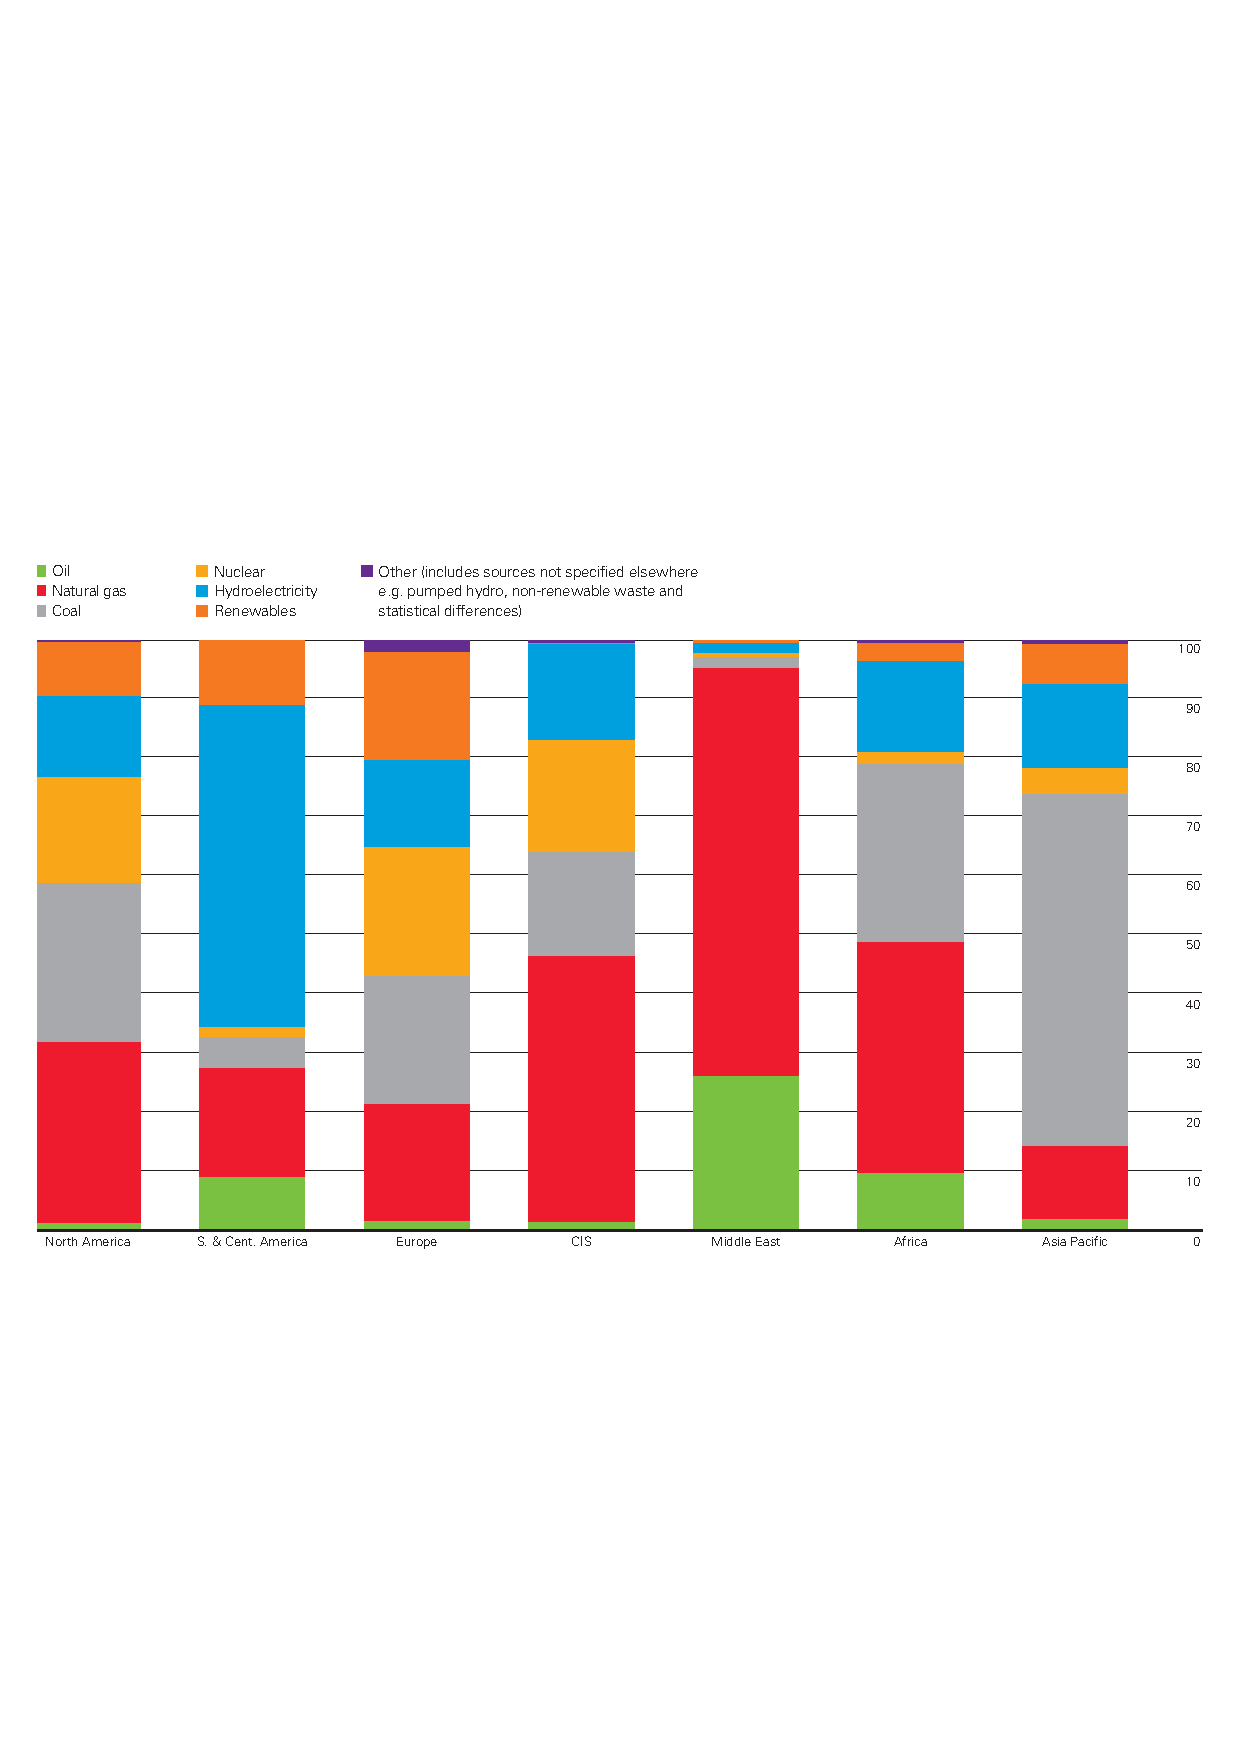
\includegraphics[width=\textwidth]{\figpath/Fig_cap_introduction/Energy_by_continent_2}
	\end{minipage}
		\begin{minipage}{.50\textwidth}
		(b) \\
		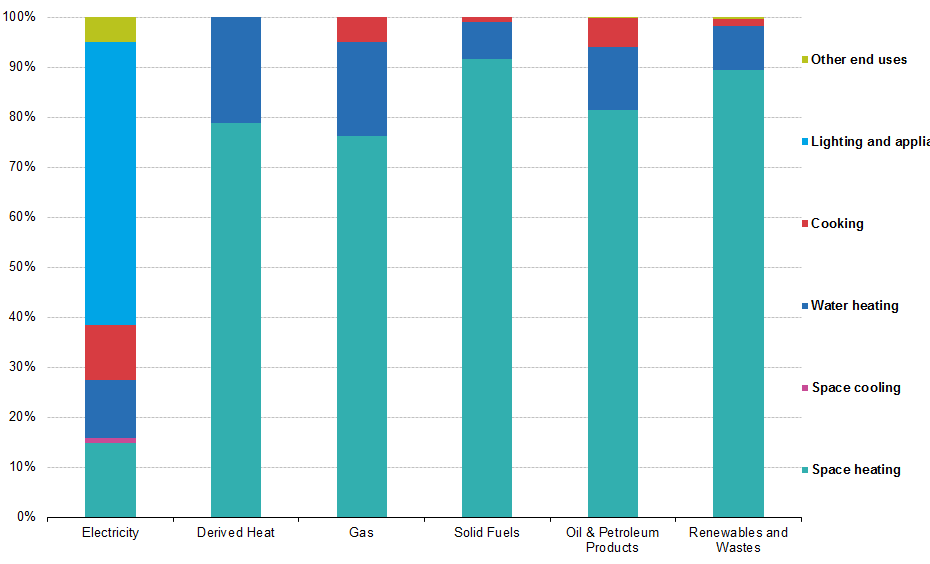
\includegraphics[width=\textwidth]{\figpath/Fig_cap_introduction/Energy-residential-EU}
	\end{minipage}
	\caption{(a) Electricity generation by different energy sources in 2017 by different continent. (b) Energy use repartition in a residential buildings in Europe.}
	 \label{fig-Energ-cons}
\end{center}	
\end{figure}

Furthermore, even though solar or wind energy are now operational, their main drawback remains their availability that not necessarily match to consumers demand.
Solar energy is not available during the nights for example, while wind energy is intermittent over the year.
Yet, the energy demand varies with time and the energy suppliers have to meet this demand.
An efficient solution to this discrepancies of availability and demands problem is the use of energy storage systems.
The idea is to store the energy at one time in one form or another and release it latter for a particular need, since energy availability and demand rarely concur.
The energy storage technologies are hence an essential point in the domain of the alternative energy.
The later can be divided into five classes:
magnetic, biological, chemical, mechanical and thermal energy storages.
The main feature of the aforementioned energy storage technologies relies on energy charging and discharging process.
In most cases however, thermal energy is the energy form widely used.
Even the electricity generation is monitored by heat generating high temperature and high pressure.
Storing thermal energy is thus an efficient and fundamental way to store the energy.
It can be realised by rising the substance's temperature (sensible heat energy storage) or by changing the substance's phases (latent heat energy storage).

Research on passive heat storage system have attracted many considerations lastly, namely interest on Phase Change Material (PCM) as latent heat energy storage have arisen.
PCM are used to store heat during the melting of the materials and releases later the stored heat during the solidification process.
At present, the latent heat storage technologies are proven as an effective solution to decrease the use of fossil fuel and in the same time increase the energy usage efficiency.

Moreover, taking advantage of the high value of the latent heat of solidi-liquid transformations, PCMs are also widely encountered in thermal regulation in buildings to reduce overheating.
In summer, PCMs are used to absorb the excessive solar radiation heat and maintain a bracing indoor ambience.
PCM with a temperature of fusion close to the ambient temperature is generally used to ensure a melting during the daytime and a solidification during the nighttime.
During winter however, PCMs can be used to store heat generated by electrical heating system during the night and then release it in the daytime.
Latest announcement of the french ministry of ecological transition, detailing the repartition of the energy consumption in different domains, indicates more than $35 \%$ of the total energy being consumed by residentials and commercial buildings. Details about energy consumptions in 2017 are shown in Tab. \ref{tab-french-min}.
This important energy demand in buildings is mostly due to the increasing need of comfort conditions and the associated market penetration of more cooling/heating systems.
More than $60\%$ of the total energy consumption in residential sector is dedicated to space heating (see Fig. \ref{fig-Energ-cons}b).
Research towards energy-efficient building is thus rising to reduce heating and cooling demand.
The use of efficient insulation is the key of energy conservation in residential buildings.

\begin{table}
	\begin{center}
		\begin{tabular}{ccccc}
			Agriculture & Buildings & Industry  & Transportation & Other  \\ \hline
			4.5 & 41.8 & 26 & 43.8 & 4.5 \\
		\end{tabular}
	\end{center}
	\caption {The energy consumed by different domain in France in 2017, in million tonne of oil equivalent. French ministry of ecological transition.}
	\label{tab-french-min}
\end{table}

A wide range of recent PCM applications are know available in the literature, ranging from metal casting to passive temperature control devices (e. g. for modern portable electronics), and several authors have carried out investigation into a wide range of PCMs.
The choice of an appropriate material for a specific application depends indeed of many criteria, such as the operating temperature range, the thermal conductivity, the costs, etc.
PCM are generally classified into three classes: organic, inorganic and eutectic.
A target application area for some PCM are drawn in Tab. \ref{tab-PCM-app}.
The main operating temperature range can be assorted by three groups. First, $0$ to $65 ^o C$ for thermal storage used in domestic heating/cooling or for thermal storage of solar energy. Paraffins and water are used for such applications.
Second, $80$ to $120 ^o C$ for the cooling of systems with generator temperature of less than $120 ^o C$ purpose.
Finally, greater than $150 ^o C$ for the heat storage in solar power plants based on parabolic trough collectors and direct steam generation.


\begin{table}[h!]
	\begin{flushleft}
		\begin{tabularx}{\linewidth}{cXX}
					Temperature range & PCM & Target application area \\ \hline \hline
			0 - 65 $^o C$ &    Paraffins (-3 to 64 $^o C$), water / ice  (0 $^o C$), stearic acide  (41 - 43 $^o C$), {n-octadecane  (27.7 $^o C$)}   &   Storage for domestic heating/cooling. Passive storage in bio-climatic building/architecture. Thermal storage of solar energy. Application in off-peak electricity for cooling and heating. Protection of electrical devices.\\ \hline
			%80 - 120 $^o C$ & Erythritol (117.7 $^o C$), RT100  (99 $^o C$),  $MgCl_2 6H_2 O$& \\ \hline
			80 - 120 $^o C$ &    Erythritol (117.7 $^o C$), RT100  (99 $^o C$), $MgCl_2 \, 6H_2O$  (116.7 $^o C$)   &   Storage for the hot-side of $LiBr/H_2O$ absorption cooling system with generator temperature requirements of less than 120 $^o$C\\ \hline
			$ > 150 $ $^o C$ &    $NaNO_3$ (310 $^o C$), $KNO_3$  (330 $^o C$), $NaOH$  (318 $^o C$),  $KOH$  (380 $^o C$), $ZnCl_2$  (280 $^o C$)  &   Storage for solar power plants based on parabolic trough collectors and direct steam generation.\\ 

		\end{tabularx}
	\end{flushleft}
	\caption {Target application area for some PCM studied in the literature.}
	\label{tab-PCM-app}
\end{table}

\section{Purpose of the thesis}
The purpose of the present work is to investigate numerically solid-liquid phase-change systems.
The investigation tool used in this thesis is the open-source software FreeFem++ \citep{freefem,hecht-2012-JNM}.
A high accuracy numerical model using a Newton method with an adaptative finite element is used to simulate phase-change system with natural convection.

A first work on the numerical simulation of phase-change problems using finite element method have been carried out by \cite{dan-2014-JCP}.
A Newton method was used to solve the Navier-Stokes-Boussinesq system of equations with an enthalpy model for the phase-change using a single domain approach.
A first-order scheme was applied for the time discretization and a viscosity-based method was used to deal with the single domain approach.
Two-dimensional square cavity domain was mainly studied.

In the present work, the main objectives are listed as follows:\\
(i) use a second order scheme for the time discretization and a P$_2$ finite element for the temperature,\\
(ii) implement a Carman-Kozeny model, in addition to the viscosity-based approach, to annihilate the velocity in the solid region,\\
(iii) simulate more complex geometries: circular PCM, highly distorted mesh geometry, rectangular PCM, \\
(iv) simulate the challenging melting-solidification cycle of PCM, \\
(v) carry out a finite element tool box using FreeFem++ software to simulate phase-change with natural convection problems, \\
(vi) simulate three-dimensional configurations.

\subsection{Existing method for modeling phase-change materials}
Solid-liquid phase-change is known to be a tough problem, be it theoretically or numerically.
The non-linear time-dependent evolution of the interface would raise for example a major issue.
Indeed, the strong coupling between the temperature and the velocity field makes the calculation of the position and the velocity of the interface very difficult.
From a mathematical point of view, actual chalenge is about the derivation of a realistic theoretical framework, using transport equations for different involved quantities (velocity, temperature, concentration, density, etc.).
As far as the one-dimensional Stefan problem is concerned, the existence and the uniqueness of the solution was proven \citep{rubinstein1947solution,evans1951note,douglas1957uniqueness}.
Moreover, exact solution for non-isothermal transitions and multi-dimensional problems were discussed by \citep{elliott1987error,cho1969heat} and both analytical and approximated solutions were given by \citep{tarzia2011explicit}. 
Furthermore, for the progressive consideration of the natural convection in phase-change problems, one can see the historical review by \citep{yao1989melting}. \\
Concerning the numerical modeling, the existing method in the literature can be divided into two main categories:
multi-domain or single-domain methods.
Each methods are appropriate for either pure fluid (pure material) or multi-phase (homogeneous mixtures) problems. \\
The multi-domain methods can be classified into two families:
the moving grid or the eulerian approaches. 
The front tracking methods, the mapping methods, the transformed grid methods or the front fixing methods belong to the moving grid families \citep{sparrow1977analysis,gupta2000moving}.
The main idea is to track explicitly the interface and thus to solve separately the liquid and the solid phases.
The interface is governed by energy balance, corresponding to a boundary condition for each phases. 
However, the eulerian methods aim to follow implicitly the interface by the mean of a new equation used to reconstruct its position.
The front fixing methods or phase fields methods are examples of such approaches.
The essential feature is that the interface is diffuse, 
at the example of the phase field methods (PFM). 
In PFM the interface is identified through a phase field variables $\phi$, involving in a free energy equation which is minimized. For a comprehensive review of these methods, see \citep{fix1982phase,davis2001theory,boettinger2002phase,singer2008phase}.\\
In contrast with multi-domain methods, single-domain methods (or enthalpy methods) solve a unique system of equations throughout the domain. 
Now the interface is neither track explicitly, nor implicitly, but is instead considered a posteriori from the computed temperature field.
The main feature of the method is about the formulation of the energy equation, which can be separated into two classes:
the enthalpy-based formulations or the temperature-based formulations.\\
First, the enthalpy-based formulations \citep{eyres1946calculation,rose1960method,bhattacharya2014enthalpy} aim at solving the enthalpy from the usual energy equation, and then from outer iterations until convergence, the temperature is updated from a temperature-enthalpy coupling model. 
A second variety consists of rewriting the energy equation with enthalpy terms only \citep{rady1996natural,hannoun2003resolving}.\\
Second, the temperature-based formulations consider the enthalpy as the sum of the latent and the apparent heats in the energy equation. 
The latent heat can be thus treated either by heat capacity coefficient methods \citep{gau1984melting,szekely1970effect,chiesa1974natural} or by heat source term methods \citep{Tenchev2005,swaminathan1997towards,dan-2014-JCP}.
The advantages and the drawbacks of each approaches were discussed in detail by \cite{konig2017comprehensive}.
By comparing several fixed-grid methods, they have concluded that enthalpy based formulations using the usual energy equation and the temperature-based formulations using heat source term approach were the more accurate and robust methods. 

It is worth noting that two other methods very different from the previous ones also exist in the literature:
the lattice boltzmann methods and the meshless methods.
The lattice boltzmann methods are derived from the lattice gas automata model: the behaviour of the particles are governed by a kinetic model, which is averaged to obtain macroscopic behaviour \citep{frisch1986lattice,luo2015lattice,gong2015numerical}.
The meshless methods use an arbitrary number of nodes, without mesh as suggested by their names, in which interpolations are done to approximate the solution. A more complete review is given by \cite{atluri2002meshless}.

In the single domain method, solving the same system of equations on the entire domain leads to a further difficulty.
Techniques to bring the velocity to zero in the solid region as to apply the momentum equation in the solid part are needed.
Three methods are mainly applied to force the behaviour of the velocity in the vicinity of the phase change interface:
the switch-off techniques, the variable viscosity methods and the Darcy source approaches.\\
In the first case, the switch-off techniques are the most straightforward approaches consisting simply of overwriting the velocity in the solid to be zero.
The solid and the liquid regions are identified through the representative latent heat of an element of the numerical discretization.
The main drawback is that this approach is known to produce oscillations and instabilities or even convergence issues.\\
In the second case, the variable viscosity method considered the viscosity $\mu$ to be function of the temperature: in the mushy region, the viscosity rises to a large value. 
Thus, the velocity is inhibited and becomes negligible in the solid region.
Difficulty is about defining the increasing function with real physical basis.\\
In the last case, the Darcy source or the Carman-Kozeny approaches, modeled the mushy region as a porous medium. 
This has the effect of vanishing the velocity through the mushy zone and goes to zero in the solid phase. 
It is worth to mention that this last approach has a physical significance.

\subsection{Present numerical approach for modeling phase-change materials}
In this thesis, we use an enthalpy method with a temperature-based formulation using heat source term approach to simulate phase-change systems with convection.
The natural convection flow in the liquid phase is simulated by solving the full incompressible Navier-Stokes equations with Boussinesq approximation.
A Carman-Kozeny type penalty model is applied to ensure a zero velocity value in the solid region.
The main feature of our numerical approach is the use of an adaptive finite element method to accurately track the solid-liquid interface.
Single domain method requires actually a fine mesh near the phase change front in order to capture the large enthalpy gradient. 
The smaller the phase change interval the narrower the mushy region and the more refined the mesh should be.
Yet applying a fine mesh in the whole domain would increase considerably the computational time.
Hence, we introduce a FE method with time-dependent mesh adaptivity by metric control that is  effective for a large range of phase-change systems with convection, from melting to solidification. The proposed mesh refinement strategy has the capacity to take into account different metrics and thus the ability to refine the mesh in different regions of interest in the computational domain. In particular, we show that the method is able to simultaneously track several interfaces in the domain.\\ %, a feature that was not present in previous mesh refinement algorithms.\\
The nonlinear system of equations are solved by means of a Newton algorithm.
A fully-implicit Newton method for the phase-change system based on a finite-element formulation of the Navier-Stokes equations has been derived by \citep{dan-2014-JCP}.
The advantage of this formulation is to  permit a straightforward implementation of different types of non-linearities in the system of equations.

 %Numerical methods based on standard finite elements are less represented in this field. To the best of our knowledge, no finite-element programs exist in the CPC Program Library for the phase-change systems simulation. The purpose of this paper is thus to distribute a finite-element solver for computing the 2D incompressible Navier-Stokes equation with Boussinesq approximation.
 The code was built as a toolbox for FreeFem++ \citep{hecht-2012-JNM,freefem}, which is a free software (under LGPL license) using a large variety of triangular finite elements  (linear and quadratic Lagrangian elements, discontinuous P$_1$, Raviart-Thomas elements, etc.)  to solve partial differential equations. FreeFem++ is an integrated product with its own high level programming language and a syntax close to mathematical formulations, making the implementation of numerical algorithms very easy. Among the features making FreeFem++ an easy-to-use and highly adaptive  software we recall the advanced automatic mesh generator, mesh adaptation, problem description by its variational formulation, automatic interpolation of data, colour display on line, postscript printouts, etc. FreeFem++ community is continuously growing, with  thousands of users all over the world.

\section{Thesis plan}
Chapter \ref{chap-NSB} sets the mathematical and physical basis of the numerical system used to simulate phase-change problems involving natural convection flow.
We present in detail the incompressible Navier-Stokes-Boussinesq equation and the single-domain approach to solve the same system of equations throughout the whole domain.
The enthalpy method, modeling the phase-change phenomenon is presented first.
The Navier-Stokes equation with Boussinesq approximation to simulate the natural convection in the liquid flow is then developed.
Finally, the final non-dimensional system of equations is described in detail with a discussion about the Carman-Kozeny model used as a penalty term in the momentum equation.

Chapter \ref{chap-FEM} is devoted to the numerical algorithm for solving the numerical system presented previously.
The finite element algorithm we have developed in this work is first presented in detail: time integration scheme, finite element discretization and the Newton method.
The characteristics Galerkin method, an alternative for the treatment of non-linear term in the momentum equation, is also presented.
Then, we describe the mesh adaptivity by metric control, which is a standard function offered by FreeFem++.
Some theoretical tests to assess for the accuracy of our numerical method is also presented.
The space and the time convergence orders are demonstrated using the Burggraf flow and a manufactured solution designed for the incompressible Navier-Stokes equation.
The structure of the new finite-element toolbox for the simulation of PCMs is also described.
The program architecture and the parameter details are presented.
Finally, the domain decomposition method used for large scale simulation is described;

A first validation of our numerical method is addressed in chapter \ref{chap-NATCONV}.
The capability of the code to deal with linear and non-linear form of the buoyancy force in the Boussinesq approximation is first tested.
The natural convection of air and water in a two-dimensional square cavity are tested.
Differentially heated cavity (horizontal $\nabla T$) configuration is used to compare our results with benchmarks solution existing in the literature.
Three-dimensional simulations of the natural convection of air is also presented.
For both two and three-dimensional configurations, qualitative and quantitative validations are provided.

Once the capability of our algorithm to deal with natural convection issues was demonstrated, much more attention to phase-change problem is paid.
Numerical simulation of PCM is considered in chapter \ref{chap-MELTING}.
Numerical and physical analysis are described in detail.
The octadecan PCM is considered first to validate our code with experimental and numerical existing results in the literature.
Accurate comparison is carried out for the differentially heated cavity case, by considering different size of the cavity and different temperature difference between the hot temperature and the temperature of fusion, which are the main parameters monitoring the natural convection in the melting PCM.
Analysis of the time evolution of some physical parameters, such as the Nusselt number, the liquid fraction, the accumulated heat input and the time evolution of the melting are provided in detail through a scaling analysis.
Then, several PCM container geometries are simulated to prove the robustness of our numerical method.
Finally, numerical simulation of three-dimensional configuration is presented.

Chapter \ref{chap-SOLIDIFICATION} presents the numerical simulation of a full cycle melting/solidification of a PCM. 
Two solidification fronts have to be tracked and make the case very challenging.
A differentially heated cavity case and a circular PCM with inner heated tubes are studied.
A comparison on the influence of the Rayleigh number during the melting and the solidification process is emphasized, since both cycles are not driven by the same mechanism.



